
% SECCIÓN: CÓMO MOLA Y FUNCIONA NUESTRA IMPLEMENTACIÓN, QUE ES EL FOCO DEL PAPER
% 
% TODO: Poner que a pesar de que el ejemplo descrito no es real ha sido for the sake of clarity, pero 
% que el sistema ha sido utilizado en supermercados y hospitales reales como está descrito en [1] noticia en castellano [2] paper nuestro hablando de ello en otra confe pasada
% 
\section{Case study}

Otsopack has been used in real scenarios both in a supermarket and in a hospital with more complex applications within
the ACROSS project\footnote{\url{http://www.acrosspse.com/across/servlet/Noticias?id=33}\linebreak
\url{http://www.acrosspse.com/across/servlet/Noticias?id=35}}. For the sake of brevity and clarity, two simple and not
implemented applications have been designed for this contribution. The aim of them is to show how the middleware
solution can be used to achieve interoperability. In order to prove the feasibility of the implementation in limited
devices, times measured in real sensors are used.

For the case study, we will model two different applications: \textit{otsoSecurity} and \textit{otsoHomeAutomation},
which have not been implemented.

\subsection{Security}

A security company can develop an application which monitors different parameters such as the temperature, the humidity
or the $CO_2$ concentration with different sensors deployed over an industrial facility. Whenever any of this measures
go
beyond a determined threshold, the company needs to take the proper action. To answer to the potential risks the
application
creates tasks with different priorities: when a unimportant parameter is outside the expected boundaries the application
can write a low priority task for the security manager into the space (e.g. the $CO_2$ is slightly higher than the
normal one),
but to warn about an emergency to the users in the facility a high priority one can be written (e.g when they must leave
the building). Then, the message is consumed by different actuators according to its priority (e.g. in the manager's
phone in a less intrusive manner or through visual or auditory alarms over the building).

The company can also develop a simpler version of the same application for the workers' personal mobile phones to ensure
that they are warned even if the alarms of the main application fail. To implement both versions of the application,
commonly used ontologies such as SSN (Semantic Sensor Network Ontology) or SWEET (Semantic Web for Earth and
Environmental Terminology) can be used, storing and sharing the triples detailed in Listing~\ref{lst:security} in a
graph.

\begin{lstlisting}[label=lst:security,caption=Sample triples provided by a $NO_2$ sensor deployed in the facility.]

Subject       Predicate                Object

wot:meas1     rdf:type                 ssn:Observation
wot:meas1     ssn:observedProperty     sweet:NO2
wot:meas1     ssn:observationResult    wot:outpt1
wot:outpt1    ssn:hasValue             wot:val1
wot:val1      ssb:QuantityValue        17
wot:val1      dul:isClassifiedBy
                     muo-ucum:microgram-per-cubic-meter
...           ...                     ...
\end{lstlisting}


\subsection{Home automation}

On the one hand, a room has been populated with several kind of sensors connected to XBee sensors\footnote{\url{
http://tinyurl.com/xbee-sensors}} with an IP gateway\footnote{\url{http://tinyurl.com/connectportx2}},
FoxG20\footnote{\url{http://www.acmesystems.it}} embedded platform connected to sensors and to an actuator.
Besides, an Android application could be performed to semantically store the user's temperature preferences. An
independent
node (master node) continuously checks the room temperature using \textit{read primitive} to get the first available
graph
where the last measure is defined (no matter which device provides that information) and the user's desired temperature.
When the second one is below the first one, it generates a ``decrease temperature during a certain period'' task which
can
be consumed by different independent worker nodes. In this case, the FoxG20 periodically checks just for orders it can
fulfill and it understands and consumes them with a \textit{take primitive}.

Once again common ontologies such as SSN (Semantic Sensor Network Ontology), MUO (Measurement Units Ontology) or RECO
(RECommendations Ontology) are used to express these relations. Sample triples provided by the mobile phone can be found
in Listing~\ref{lst:home-automation}.

\begin{lstlisting}[label=lst:home-automation,caption=Sample triples stored by the Home Automation application.]

Subject       Predicate                Object

ud:aigomez    reco:desireTowards       ud:pref1
ud:pref1      rdf:type                 reco:Preference
ud:pref1      ssn:observedProperty     swt:Temperature
ud:prefm      ssn:observationResult    ud:dout1
ud:dout1      ssn:hasValue             ud:dVal
ud:dVal       ssn:QuantityValue        20
...           ...                      ...
\end{lstlisting}


\subsection{Interoperability}

\begin{sloppypar}
Given that both systems use a common ontology called SSN, and through Triple Spaces they can be using a common space,
whenever the Security application asks for triples matching a template \codigo{?s rdf:type sweet:Temperature}, the Home
automation application would return that \codigo{wot:mes3 rdf:type sweet:Temperature} along with other information
stored in that graph. Therefore, the Security application would be able to retrieve information from another application
it does not even know. In the same way, it is feasible that the Home automation application also retrieves information
stored by the Security application in the same or other nodes.
\end{sloppypar}

The key for this interoperability process is that both applications are using the same language, since both are using
the same concepts of the same ontologies (e.g. SSN). Although this can be achieved mapping concepts from two different
ontologies with a semantic web reasoner through the \codigo{owl:sameAs} property, it is habitual to use common
ontologies. Furthermore, since all the applications should be interested in retrieving data from other potential ones,
the developers should be willing to employ widely used ontologies to ease the information exchange among applications.

\subsection{Feasibility in embedded devices}

Finally, one of the challenges of Otsopack was to support limited devices such as low cost sensors. In order to do so,
two sensors are used: FoxG20\footnote{http://www.acmesystems.it} and XBee sensors with an IP
gateway\footnote{http://tinyurl.com/connectportx2gateways}. XBee can only be programmed in Python, so a subset of the
protocol was implemented in this language, only supporting that other nodes access sensor information in the space. 

Therefore, the rest of the nodes located in the shared space would be able to query the space and the sensors would
return the information. The requests performed by Android phones or PCs with Otsopack do not deal with the sensors in a
particular way, neither the Space Managers or other Otsopack components. They only query for certain information to the
space, and the sensors return the information if the query matches the information they contain.

To evaluate if this lightweight implementation of Otsopack fits, time measurements have been taken on both sensor
platforms under different levels of stress (from 1 concurrent request to 35), and they have been compared with a regular
PC running Otsopack (Java version), as shown in Figure \ref{fig:deviceComparison}. The results show that these sensors
can support a wide number of concurrent requests using this protocol, which should be enough in the described
scenarios. In any case, the design of the particular application should take into account the limits shown in the
figure.


% TODO: should we say something such as "the implementation required a few hundred lines of Python code" or so?
% Something to say "it was really small"

% \begin{figure}
% \centering
% 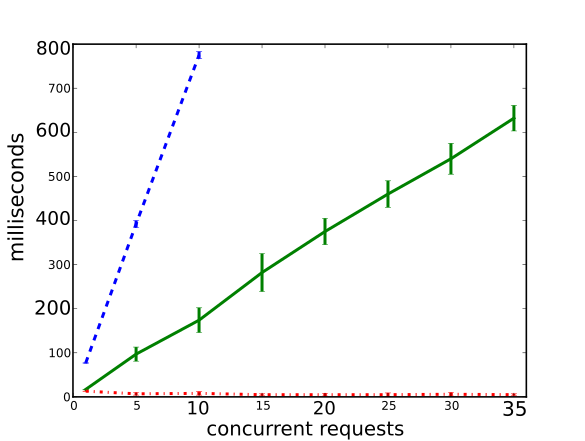
\includegraphics[width=3in]{images/device_comparison.png}
% \label{fig:deviceCompatison}
% \caption{Time measurement comparison among XBee sensors, FoxG20 and a regular computer}
% \end{figure}




\InsertFig{device_comparison}{fig:deviceComparison}{
  Response times measured in different embedded devices
}{
  The dash-dotted line represents the regular computer, the solid line the FoxG20 and the dashed line the XBee.
}{0.7}{}


\begin{table}[htbp]
    \caption{Mean of the measurements taken in different devices with the standard deviation ($\sigma$) in parenthesis.}
    \centering
    \begin{tabular}{|c|c|c|c|}
      \hline
      Concurrent & XBee & FoxG20 & Regular \\
      requests   &  & &  computer \\
      \hline
      1  &  77 (1)	&  17 (0)  &  13 (0) \\
      5  & 392 (8)	&  97 (16) &   7 (3) \\
      10 & 775 (8)	& 174 (28) &   8 (4) \\
      15 &  -	& 282 (43) &   5 (2) \\
      20 &  -	& 375 (30) &   5 (3) \\
      25 &  -	& 460 (30) &   5 (4) \\
      30 &  -	& 540 (35) &   6 (4) \\
      35 &  -	& 632 (29) &   5 (2) \\
      \hline
    \end{tabular}
    \label{tab:timeMeasures}
\end{table}